\chapter{Begriffe}
		\section{Point Cloud}\label{app:point_cloud}
			Eine Point Cloud (Punktwolke) ist eine Menge von Punkten im 3D Raum. Die Punkte sind weder miteinander verbunden, noch enthalten sie Informationen über Orientierung oder benachbarte Punkte. Die meisten 3D Scanner produzieren Point Clouds, die zu einem Mesh weiterverarbeitet werden können.
			Sind die Punkte dicht beieinander, spricht man von einer \emph{dense} (dicht) Point Cloud. Ansonsten nennt man sie \emph{sparse} (licht, locker).
			[TODO: Bild]
		
		\section{Mesh}\label{app:mesh}
			Verbindet man mehrere Punkte einer Point Cloud zu einer Fläche, meist zu Dreiecken, enthält man ein Mesh. Dies hat eine klare Orientierung und setzt Punkte in Verbindung mit ihren Nachbarn. Enthält ein Mesh keine Löcher, nennt man es \emph{watertight} (wasserdicht).
			[TODO: Bild]
		
		\section{Orthofoto} \label{app:orthofoto}
			Fotos einer üblichen Kamera, die nach dem Prinzip einer Lochkamera funktionieren, projizieren alle Lichtstrahlen, die durch den Brennpunkt fallen, auf die Bildfläche. Siehe \autoref{app:pinhole}.
			
			Erstellt man einen Plan oder Aufriss, verwendet man nicht die Projektion einer Lochkamera, sondern eine orthographische Projektion (Parallelprojektion, siehe \autoref{app:ortho_img}). Ein solches Bild kann durch Rektifizieren von normalen Fotos erreicht werden, erfordert aber meist manuelle Arbeit und kann zu Artefakten im entzerrten Bild führen.
			
			Der Vorteil von Orthofotos ist, dass sie wie ein Plan verwendet werden oder als Vorlage für solche dienen können.
			
			\begin{figure}
				\begin{subfigure}{0.5\linewidth}
					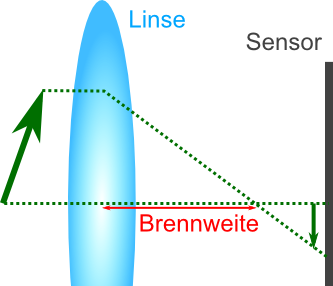
\includegraphics[width=\textwidth]{lense_pinhole}
					\caption{Schematische Darstellung einer gewöhnliche Kamera mit Linse}
					\label{app:pinhole}
				\end{subfigure}
				\hspace{0.2\linewidth}
				\begin{subfigure}{0.5\linewidth}
					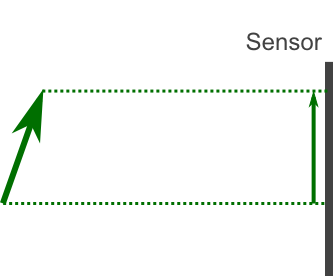
\includegraphics[width=\textwidth]{lense_ortho}
					\caption{Schematische Darstellung eines Orthofotos}
					\label{app:ortho_img}
				\end{subfigure}
			\end{figure}

		\section{Digitales Höhenmodell} \label{app:dtm}
			Ein digitales Höhenmodell versucht in einer 2D Darstellung die Information der fehlenden dritten Dimension darzustellen. Dazu können Höhenlinien oder auch Farben verwendet werden.
			[TODO: Bild]
			
\chapter{DRONARCH verwenden}
	\section{Tipps zum Aufnehmen von Fotos}\label{app:tip_foto}
	\section{Parameter}\label{app:param}
	
\chapter{Implementierung} \label{app:imp}
	\section{Computer Vision} \label{app:imp:comp_vis}
	
\chapter{Vergleich mit Agisoft PhotoScan}\label{app:photoscan}
	Das Programm PhotoScan von Agisoft\citeu{agisoft} implementiert die selben Schritte wie \dronarch\ und wurde in der Archäologie schon mehrfach verwendet und dokumentiert\citeu{arch:laser_vs_dense_stereo, ARCM:ARCM667, ARP:ARP399, DeReu20131108,  altai}. Ein Versuch 
	